\begin{abstract}
AI agents increasingly operate as part of interacting systems rather than in isolation. As agents exchange information and jointly make decisions, their interactions can improve collective reasoning but may also produce herding, polarization, or amplify shared biases.
Understanding and predicting these collective dynamics is therefore important for designing effective and aligned multi-agent systems. Here, we study over 10,000 communities of language-model agents that repeatedly exchange messages and revise their opinions across objective mathematics questions and subjective political statements. Despite substantial diversity in possible behavior, the individual and group dynamics can be represented by three characteristic regimes: indifference, polarization, and consensus. AI agents start indifferent and build conviction as they interact. On objective questions, communication improves collective accuracy, while on subjective questions it often drifts group opinions toward the right in the political spectrum. We explain these observations with a statistical-mechanics formalism in which agents stochastically favor lower social pressure. Given only initial opinions, our model predicts individual trajectories, outperforms all standard baselines, generalizes to unseen community graphs, and reproduces the observed group archetype distributions. Our fitted model parameters reveal the mechanics underlying our key observations: i) communities operate below the critical social temperature, which explains conviction buildup; ii) attractive ties outweigh repulsive ones, which favors consensus; and iii) agents holding the correct answer exert the strongest pull, which drives truth-seeking. Overall, our results demonstrate that collective behavior of AI agents, like that of other complex systems, follows compact and predictive dynamical laws.

\end{abstract}

\begin{figure}[h]
    \centering
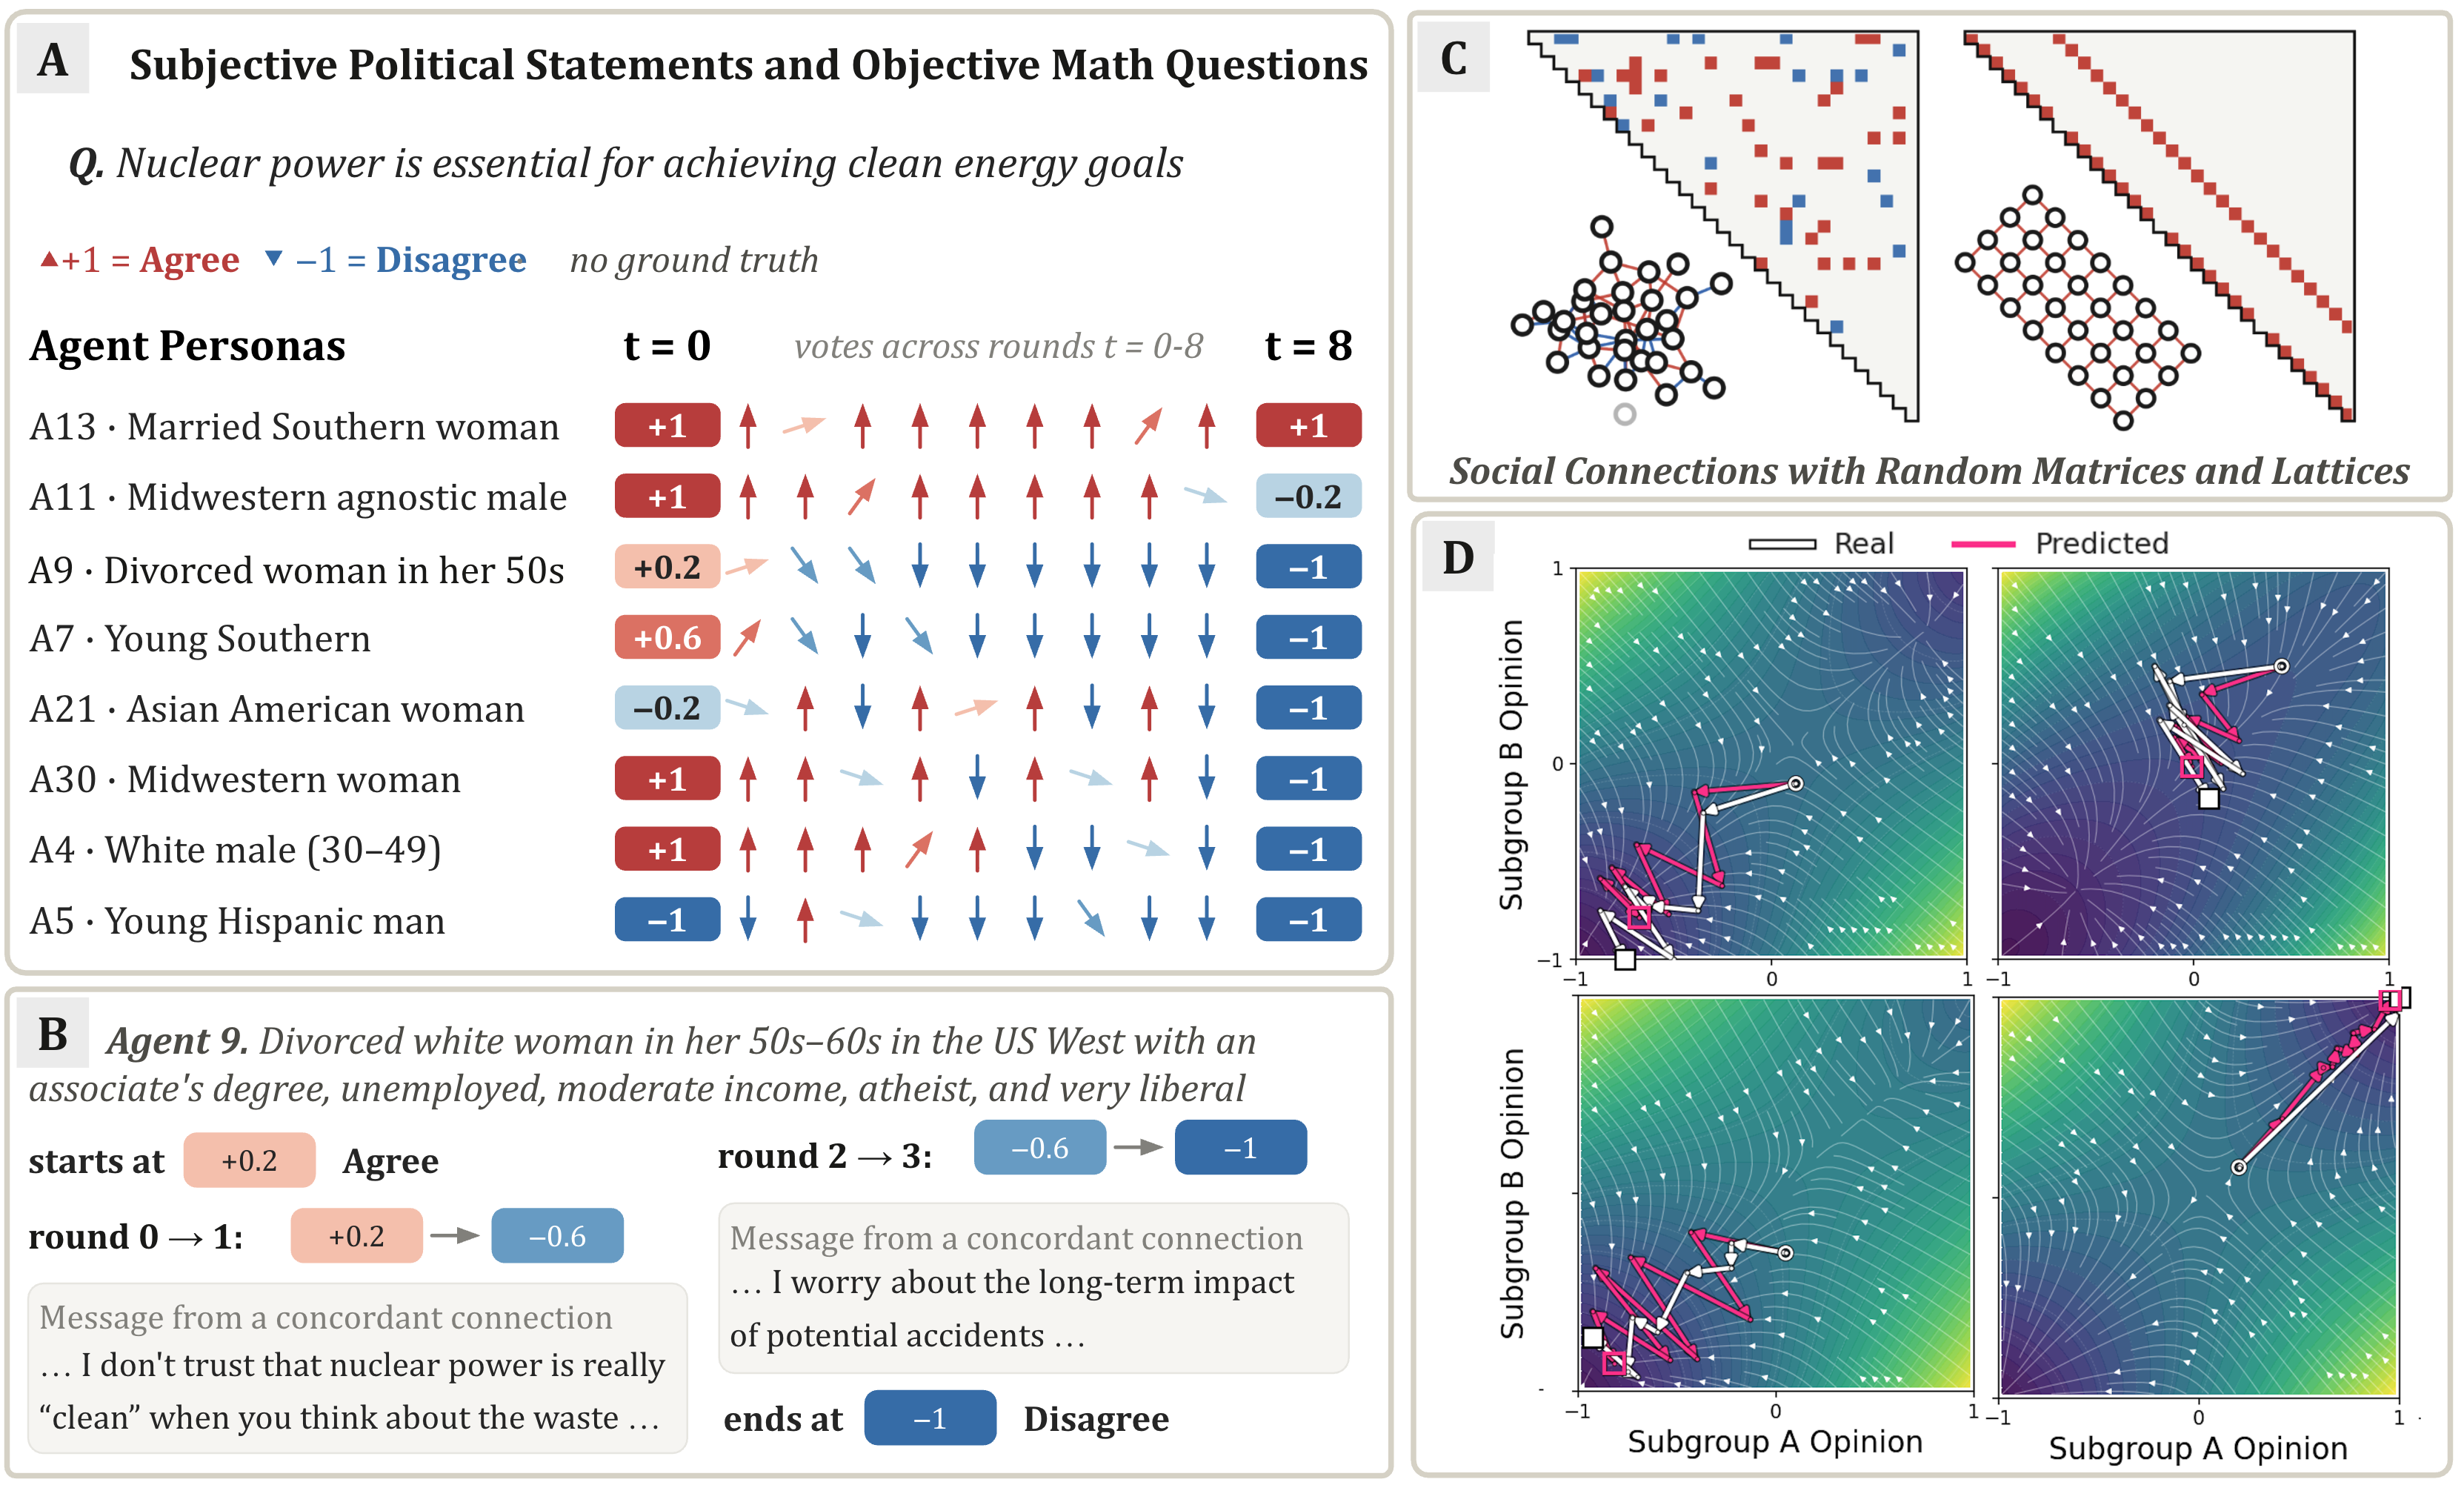
\includegraphics[width=0.99\textwidth]{main/Figures/main_01_teaser_opinion_flow.png}
\caption{\textbf{A. Opinion Updates.} Opinions of eight agents over eight rounds of message exchange, from their initial opinion at $t=0$ to their final opinion at $t=8$; agents start out mostly agreeing on one side and end up on the other. \textbf{B. Message Exchange.} Messages received by the agents and the opinion changes that followed. \textbf{C. Communication Networks.} Two of the four families of communication networks (random matrices, square lattices) shown as the signed adjacency $J$ as a heatmap in one corner triangle (blue $-1$, white $0$, red $+1$) and as a node-link diagram. See Appendix \ref{apdx:communication_networks} \textbf{D. Prediction.}  Each panel is one
group of $N$ language-model agents interacting about a question over eight rounds. We split the agents into two subgroups based on their opinion at $t=0$ (see Appendix \ref{apdx:f1} for details). White arrows are the real (observed) opinion changes, and the pink lines are discrete opinion updates predicted with our fitted model rolled out from the initial opinions at $t=0$. The background shows the energy in colors and predicted flow, which describe continuous limit, in streamlines.}
     \label{fig:1_intro}
\end{figure}


